
% !TEX root = main.tex

\begin{figure}[t]
\vspace{-1.5cm}
\begin{minipage}{0.34\textwidth}
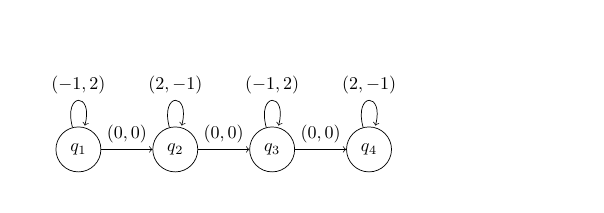
\begin{tikzpicture}[scale=0.25]
\usetikzlibrary{automata, positioning}
\scalebox{0.65}{
\node[state] (q1) {$q_1$};
\node[state, right=of q1] (q2) {$q_2$};
\node[state, right=of q2] (q3) {$q_3$};
\node[state, right=of q3] (q4) {$q_4$};

\path[->] (q1) edge [loop above] node[above] {$(-1,2)$} (q1) edge node[above] {$(0,0)$} (q2); 
\path[->] (q2) edge [loop above] node[above] {$(2,-1)$} (q2) edge node[above] {$(0,0)$} (q3);
\path[->] (q3) edge [loop above] node[above] {$(-1,2)$} (q3) edge node[above] {$(0,0)$} (q4);
\path[->] (q4) edge [loop above] node[above] {$(2,-1)$} (q4);
}
\end{tikzpicture}
\end{minipage}
\begin{minipage}{0.32\textwidth}
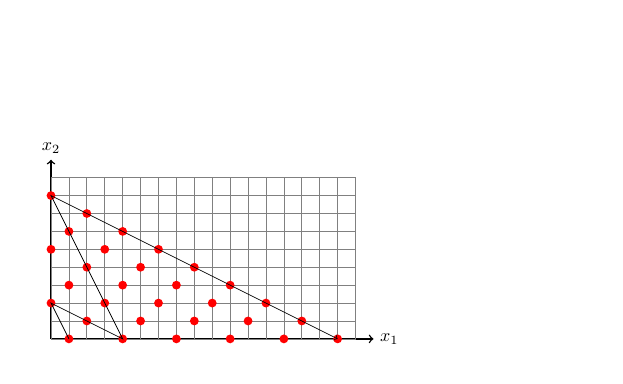
\begin{tikzpicture}[scale=0.35]
\scalebox{0.65}{
\draw[->, thick] (0, 0) -- (18, 0) node[right] {$x_1$};
\draw[->, thick] (0, 0) -- (0, 10) node[above] {$x_2$};

\draw[step=1, gray, thin] (0, 0) grid (17, 9);

\foreach \x in {1,4,7,10,13,16} \fill[red] (\x,0) circle (7pt);
\foreach \x in {2,5,8,11,14} \fill[red] (\x,1) circle (7pt);
\foreach \x in {0,3,6,9,12} \fill[red] (\x,2) circle (7pt);
\foreach \x in {1,4,7,10} \fill[red] (\x,3) circle (7pt);
\foreach \x in {2,5,8} \fill[red] (\x,4) circle (7pt);
\foreach \x in {0,3,6} \fill[red] (\x,5) circle (7pt);
\foreach \x in {1,4} \fill[red] (\x,6) circle (7pt);
\foreach \x in {2} \fill[red] (\x,7) circle (7pt);
\foreach \x in {0} \fill[red] (\x,8) circle (7pt);

\draw[->] (1,0) -- (0,2) -- (2,1) -- (4,0) -- (3,2) -- (2,4) -- (1,6) -- (0,8) -- (2,7) -- (4,6) -- (6,5) -- (8,4) -- (10,3) -- (12,2) -- (14,1) -- (16,0);
}
\end{tikzpicture}
\end{minipage}
\begin{minipage}{0.32\textwidth}
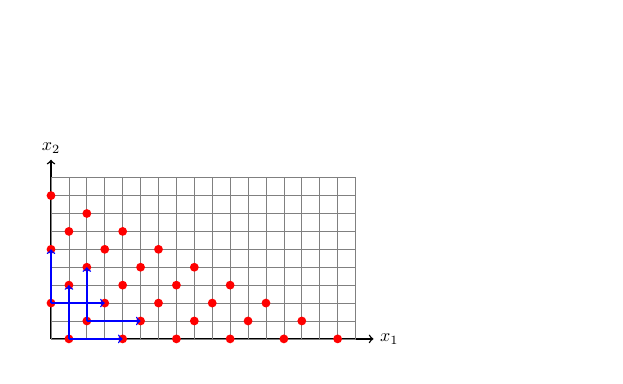
\begin{tikzpicture}[scale=0.35]
\scalebox{0.65}{
\draw[->, thick] (0, 0) -- (18, 0) node[right] {$x_1$};
\draw[->, thick] (0, 0) -- (0, 10) node[above] {$x_2$};

\draw[step=1, gray, thin] (0, 0) grid (17, 9);

\foreach \x in {1,4,7,10,13,16} \fill[red] (\x,0) circle (7pt);
\foreach \x in {2,5,8,11,14} \fill[red] (\x,1) circle (7pt);
\foreach \x in {0,3,6,9,12} \fill[red] (\x,2) circle (7pt);
\foreach \x in {1,4,7,10} \fill[red] (\x,3) circle (7pt);
\foreach \x in {2,5,8} \fill[red] (\x,4) circle (7pt);
\foreach \x in {0,3,6} \fill[red] (\x,5) circle (7pt);
\foreach \x in {1,4} \fill[red] (\x,6) circle (7pt);
\foreach \x in {2} \fill[red] (\x,7) circle (7pt);
\foreach \x in {0} \fill[red] (\x,8) circle (7pt);

\draw[->,blue,thick] (1,0) -- (4,0);
\draw[->,blue,thick] (1,0) -- (1,3);

\draw[->,blue,thick] (2,1) -- (5,1);
\draw[->,blue,thick] (2,1) -- (2,4);

\draw[->,blue,thick] (0,2) -- (3,2);
\draw[->,blue,thick] (0,2) -- (0,5);
}
\end{tikzpicture}
\end{minipage}
\caption{Left: 4-component \dvass $V_2$. 
Middle: the set $\reach_{q_4}(V_2, q_1(1,0))$ and a path $q_1(1,0) \tran q_4(16,0)$.
Right: bases 
%$A = \{(1,0),(2,1),(0,2)\}$ 
and periods 
%$P = \{(0,3),(3,0)\}$
 of an over-approximating semi-linear set $A+P^*$.}
\label{fig:zigzag}
\end{figure}

\begin{example}
For $k\geq 1$, let $V_k$ be a $(2k)$-component \dvass, where each component has just one state $q_i$
and one transition:
$(q_i, (-1,2), q_i)$ for odd $i$, and $(q_i, (2,-1), q_i)$ for even $i$.
Bridge transitions are $(q_i, (0,0), q_{i+1})$.
Figure~\ref{fig:zigzag} shows $V_2$ (left) and 
a path in $V_2$ from $s = q_1(1,0)$ to $t = q_4(16,0)$ together with 
the reachability set $\reach_{q_4}(V_2, s)$ (middle).
In general,
\begin{align} \label{eq:reachk}
X_k := \reach_{q_{2k}}(V_k, s) \ = \ \set{(x_1,x_2) \mid x_1+2x_2 \leq 4^k, \  x_1+2x_2 \equiv 1 \!\! \mod 3}.
\end{align}
Even if the size of the reachability set is 
exponential in $k$, for small $(x_1, x_2)$ it is periodic and the periods are small.
The set $X_k$ can be over-approximated by $A + P^*$ for $A = \set{(1,0),(2,1),(0,2)}$ and $P = \set{(0,3),(3,0)}$
(shown on the right of Figure~\ref{fig:zigzag}), namely for every $k\geq 1$ and $B\in\N$,
the set $X_k$ is \kanapka {$8$} {$B$}. 
For illustration, consider $Y := X_k \cap ((1,0) + P^*)$.
If $(1,0) + P^{\leq B} \subseteq X_k$ then $Y$ is a $B$-approximation
of $(1,0) + P^*$ with $\norm((1,0)), \norm(P) \leq 3 \leq 8$. 
Otherwise, there is some $(v_1, v_2) \in \big((1,0) + P^{\leq B}\big)\setminus X_k$, and
then $B$ is larger than $4^k$:
\[
%8B \geq 2(1 + 3B) \geq 2(v_1 + v_2) \geq v_1 + 2 v_2 > 
4^k < v_1 + 2 v_2 \leq 2(v_1 + v_2) \leq 2(1+3B) \leq 8B.
\]
Therefore by \eqref{eq:reachk}, each $(x_1,x_2) \in Y$ satisfies 
$\norm(x_1,x_2) = x_1 + x_2 \leq x_1 + 2x_2 \leq 4^k < 8B$, and thus
$Y$, seen as a union of singletons, is a union of 
linear sets with norm of base bounded by $8B$ and empty set of periods. 
In both cases, 
$Y$ is \kanapka {$8$} {$B$}. 
%The same intuition stays behind polynomial approximability of \dvass stated in Lemma~\ref{lem:2vass-sandwich}.
\end{example}
\section{Background}
\label{sec:background}
% \subsection{Data Contamination}
% LLMs have emerged as powerful tools, facilitating a wide range of downstream applications across various fields, e.g.,
% healthcare~\citep{zhang-etal-2023-huatuogpt,53083}, financial~\citep{yan-zhu-2025-creditllm,wu2023bloomberggpt}, Legal~\citep{wu-etal-2024-knowledge,cui2023chatlaw}, education~\citep{weijers-etal-2024-quantifying,KASNECI2023102274}, scientific research~\citep{si2024can,wysocki-etal-2024-llm}, and software development~\citep{tong-zhang-2024-codejudge}.
% However, the issue of data contamination is widely recognized in the community~\citep{golchin2024timetravelllmstracing}.
% Data contamination occurs when portions of the training data unintentionally appear in the test set, creating the illusion of superior performance. 
% \CM{Can we use symbols to formally define data contamination, maybe we can formulate a model is trained bu multiple stage, and if the model see the data in any stage of its pre-training or post training, then it is contamination}
% \TODO{formally define train data and test data, and its overlap to quantify data contamination. }
% This can lead to misleading and unreliable outcomes when the model is deployed in real-world scenarios.
% To this end, extensive research has been conducted to detect data contamination~\citep{tu2024dice} and develop contamination-free benchmarks for reliable evaluation~\citep{white2024livebench}.

\subsection{Data Contamination}

% \CM{can we remove this paragraph?} LLMs have emerged as powerful tools, facilitating a wide range of downstream applications across various fields (e.g., healthcare~\citep{zhang-etal-2023-huatuogpt,53083}, finance~\citep{yan-zhu-2025-creditllm,wu2023bloomberggpt}, legal~\citep{wu-etal-2024-knowledge,cui2023chatlaw}, education~\citep{weijers-etal-2024-quantifying,KASNECI2023102274}, scientific research~\citep{si2024can,wysocki-etal-2024-llm}, and software development~\citep{tong-zhang-2024-codejudge}). However, the issue of data contamination is widely recognized in the community~\citep{golchin2024timetravelllmstracing}.

% Data contamination occurs when portions of the training data inadvertently appear in the test set, leading to an overestimation of model performance. To formally define this, let \(\mathcal{D}_{\text{train}}\) denote the complete training dataset and \(\mathcal{D}_{\text{test}}\) denote the test dataset. In many settings, models are trained in multiple stages (e.g., pre-training and fine-tuning). If we let \(\mathcal{D}_s\) be the dataset used at stage \(s\) for \(s=1,\dots,S\), then the overall training data is
% \[
% \mathcal{D}_{\text{train}} = \bigcup_{s=1}^{S} \mathcal{D}_s.
% \]

% We define the \emph{contamination set} as the intersection of the training and test datasets:
% \[
% \mathcal{D}_{\text{contam}} = \mathcal{D}_{\text{train}} \cap \mathcal{D}_{\text{test}}.
% \]
% Contamination Ratio, 
% which represents the fraction of test data that has been seen during training, could be used to quantify data contamination:
% \[
% C = \frac{|\mathcal{D}_{\text{contam}}|}{|\mathcal{D}_{\text{test}}|},
% \]

% Data contamination can lead to misleading evaluations, as the model may appear to perform well on test data it has already encountered, thereby failing to accurately reflect its true generalization capabilities. Consequently, extensive research has been conducted to detect data contamination~\citep{tu2024dice} and to develop contamination-free benchmarks for reliable evaluation~\citep{white2024livebench}.



% \subsection{Formalization of Data Contamination}
% \TODO{Merege the two subsections}
% \TODO{Add a paragraph to highlight differences between previous survey and ours}

Data contamination occurs when LLM's training data \(\mathcal{D}_{\text{train}}\) contains information that improperly overlaps with evaluation benchmark data \(\mathcal{D}_{\text{test}}\), compromising the validity of performance measurements. We summarize existing work and provide a formal definition of data contamination.

\noindent \textbf{Exact contamination} occurs when there is any exact duplicate in the benchmark dataset 
\[
\small
\exists \, d \quad \text{s.t.} \quad d \in \mathcal{D}_{\text{train}} \text{ and } d \in \mathcal{D}_{\text{test}}
\]
In other word, there exist a data point $d$ that both in $\mathcal{D}_{\text{train}}$ and $\mathcal{D}_{\text{test}}$.
Common cases include verbatim test examples appearing in training corpora, code snippets from benchmark implementations, or documentation leaks.

\noindent \textbf{Syntactic contamination} occurs when a test data point could be found in the training dataset after  a syntactic transformation, such that
\[
\small
\exists \, d \quad \text{s.t.} \quad \mathcal{F}_{\text{syntactic}}(d) \in \mathcal{D}_{\text{train}} \text{ and } d \in \mathcal{D}_{\text{test}}
\]
where \(\mathcal{F}_{\text{syntactic}}\) denotes syntactic transformations like punctuation normalization, whitespace modification, synonym substitution, morphological variations, or syntactic paraphrasing while preserving lexical meaning.

% \noindent \textbf{Semantic contamination} occurs when there is semantically equivalent content
% \[
% \exists \, d \quad \text{s.t.} \quad \mathcal{F}_{\text{semantic}}(d) \in \mathcal{D}_{\text{train}} \text{ and } d \in \mathcal{D}_{\text{test}}
% \]
% where \(\mathcal{F}_{\text{semantic}}\) represents a transformation that preserves semantic equivalence. Examples include reworded math problems with identical solution logic, paraphrased factual questions testing the same knowledge, and cross-lingual translations.



\paragraph{Examples of each contamination}
We provide contamination examples in \tabref{tab:contamination_examples}. In the case of syntactic contamination, the test data is derived from the training data by rephrasing it with the addition of a prefix string. There is ongoing debate about whether such syntactic transformations constitute true data contamination, as it is challenging to distinguish between an LLM’s ability to recall memorized information and its reasoning capability during inference. In this work, we consider such syntactic transformations as contamination, given that some NLP applications rely primarily on syntactic information for decision-making.




\paragraph{Significance of contamination} Understanding and mitigating potential data contamination in benchmarking LLMs is significant, especially given the rapid pace of LLM development. Without a robust approach to identifying and preventing contamination, evaluations may overestimate a model’s true capabilities by inadvertently testing it on data it has already seen. This undermines the validity of benchmarks, making it difficult to assess generalization, robustness, and real-world applicability. Contaminated benchmarks can lead to misleading conclusions about progress in LLM research, influencing model comparisons, deployment decisions, and policy-making. Addressing this issue is crucial for ensuring that benchmarks provide an accurate and reliable measure of an LLM’s true ability to handle novel and unseen data.






% \subsection{LLM Training}
% Unlike traditional neural models, which explicitly separate training and evaluation data, the development of LLMs involves large-scale pre-training and post-training, significantly increasing the likelihood of overlap between the training and evaluation corpora.
% During pre-training, the model learns from vast amounts of data in a self-supervised manner. 
% LLM pre-training datasets are typically curated from diverse sources, with a significant portion obtained from the web, e.g., FineWeb~\citep{penedo2024the}.
% Since many benchmark datasets are publicly available online, there is a potential risk that evaluation data may be inadvertently included in the pre-training corpus.
% After pre-training, LLMs undergo a post-training stage to further enhance their capabilities. 
% Post-training data typically include large-scale human-annotated task datasets~\citep{mukherjee2023orca,kim-etal-2023-cot} or synthetic data generated by proprietary models~\citep{ding2023enhancing,OpenHermes25,wang2023openchat}.
% Since post-training data may contain tasks similar to those in evaluation datasets, there is a potential risk of data leakage. 
% Furthermore, as the data sources of proprietary LLMs remain undisclosed, the use of synthetic data could also inadvertently introduce evaluation data contamination.

% While developers can attempt to mitigate evaluation data contamination using retrieval-based detection methods~\citep{team2024gemini,achiam2023gpt}, the vast scale and complexity of training datasets make it difficult to fully exclude evaluation data from the training set. 
% Additionally, although many open-source models exist, a significant number still keep their training data proprietary~\cite {dubey2024llama,yang2024qwen2}.
% For model consumers, accurately assessing a model's true performance can be challenging, underscoring the importance of designing fair and reliable benchmarks.


\subsection{Contamination from LLM Training}
% \TODO{either put 2.1 as the last subparagraph or make 2.2 and 2.3 related with contamination}
Unlike traditional models with clear separations between training and evaluation data, LLMs are pre-trained on massive, diverse datasets—often scraped from the web (e.g., FineWeb~\cite{penedo2024the})—which increases the risk of evaluation data overlap. In the post-training phase, models are further fine-tuned on large human-annotated~\cite{mukherjee2023orca,kim-etal-2023-cot} or synthetic datasets~\cite{ding2023enhancing,OpenHermes25,wang2023openchat} that may resemble evaluation tasks, further compounding contamination risks. Although retrieval-based detection methods~\cite{team2024gemini,achiam2023gpt} exist, the sheer scale and complexity of training corpora make it difficult to entirely exclude evaluation data. Additionally, many LLMs keep their training data proprietary~\cite{dubey2024llama,yang2024qwen2}, complicating the accurate assessment of their true performance and highlighting the need for fair and reliable benchmarks. This opacity further exacerbates data contamination, as it impedes the community’s ability to verify and mitigate potential overlaps between training and evaluation data.


\subsection{LLM Benchmarking}
% \TODO{@Yiming: Aggregated benchmarks and domain-specific benchmarks are not listed in Tab.~\ref{tab:dynamic-benchmarks}}
% \TODO{Math, Language, Coding, Reasoning, Knowledge, Safety, Instruction Following, Reading Comprehension}
% \paragraph{Benchmarking Tasks}
% \TODO{@lzx: Explain various evaluation task type and what type of capacity these tasks evaluate, e.g., mcq, instruction following,... Leave detailed dataset name to Sec 3 and 4.} 


% ==================================
% ==================================
% ==================================
% ==================================
% ==================================


As LLMs evolve into general-purpose task solvers, it is crucial to develop benchmarks that provide a holistic view of their performance.
To this end, significant human effort has been dedicated to building comprehensive benchmarks that assess various aspects of model performance. For example, instruction-following tasks evaluate a model's ability to interpret and execute commands~\citep{zhou2023instruction,qin2024infobench,huang2024c}, while coding tasks assess its capability to generate and understand programming code~\citep{chen2021evaluating,austin2021program,jimenez2024swebench,codeforces,aider}.
Despite their usefulness, static benchmarks face challenges as LLMs evolve rapidly and continue training on all available data~\citep{villalobos2022will}. Over time, unchanging benchmarks may become too easy for stronger LLMs or introduce data contamination issues.
Recognizing this critical problem, contamination detectors have been developed to quantify contamination risks, and dynamic benchmarks have been proposed to mitigate these issues.


% For example, instruction following tasks test the model's ability to interpret and execute commands~\citep{zhou2023instruction,qin2024infobench,huang2024c}; coding tasks evaluate its capability to produce and understand programming code~\cite{chen2021evaluating,austin2021program,jimenez2024swebench,yang2024swebenchmultimodal,jain2024livecodebenchholisticcontaminationfree,codeforces,aider}; and language tasks measure proficiency in traditional NLP challenges such as inference and classification~\citep{wang2018glue,wang2019superglue,xu2020clue}. Reasoning benchmarks probe whether models can leverage everyday knowledge to make logical inferences~\cite{bisk2020piqa,sap2019socialiqa,zellers2019hellaswag,sakaguchi2021winogrande,he2024chinese}, while various knowledge tasks assess factual recall and grounding~\cite{kwiatkowski2019natural,joshi2017triviaqa,hendrycks2020measuring,suzgun2022challenging,zhong2023agieval,gema2024we,wang2024mmlu,Darioush2024ControlBench,li2023cmmlu,krishna2024fact,rein2023gpqagraduatelevelgoogleproofqa,alpaca_eval,arenahard2024}. Reading comprehension tests gauge the ability to extract and interpret information from text passages~\citep{rajpurkar2018know,choi2018quac,clark2019boolq}, and math tasks challenge the model with numerical and logical problem-solving~\citep{cobbe2021training,hendrycks2021measuring,maa2024aime,cnmo2024}. Safety benchmarks~\citep{gehman-etal-2020-realtoxicityprompts,hartvigsen2022toxigen} focus on evaluating a model's ability to avoid generating harmful or toxic content. 
% % To this end, many researches focus on building the evaluation benchmark to understand the different capabilities of LLMs. 
% Although these static benchmarks cover a broad range of tasks, many are not specifically designed to prevent data contamination and thus suffer from it. Recognizing this critical issue, dynamic benchmarks have been proposed to mitigate data contamination by ensuring a clearer separation between training and evaluation data.



% For instance, instruction following task is assessed with tasks such as IFEval~\citep{zhou2023instruction} and InfoBench~\citep{qin2024infobench}, which gauge a model’s ability to understand and execute detailed commands. Code generation and comprehension are measured through datasets like HumanEval~\citep{chen2021evaluating}, MBPP~\citep{austin2021program}, SWE-Bench~\citep{jimenez2024swebench,yang2024swebenchmultimodal}, LiveCodeBench~\citep{jain2024livecodebenchholisticcontaminationfree}, as well as competitive programming challenges featured on Codeforces~\citep{codeforces} and Aider~\citep{aider}. Traditional language understanding is evaluated by GLUE~\citep{wang2018glue}, SuperGLUE~\citep{wang2019superglue}.

% Commonsense reasoning is evaluated using benchmarks such as PIQA~\citep{bisk2020piqa}, SIQA~\citep{sap2019socialiqa}, HellaSwag~\citep{zellers2019hellaswag}, and WinoGrande~\citep{sakaguchi2021winogrande}, alongside academic challenges like ARC~\citep{clark2018think}, OpenBookQA~\citep{mihaylov2018can}, and CommonsenseQA~\citep{talmor2018commonsenseqa}. World knowledge tasks, including NaturalQuestions~\citep{kwiatkowski2019natural} and TriviaQA~\citep{joshi2017triviaqa}, test the ability to retrieve factual information, while reading comprehension is measured through SQuAD~\citep{rajpurkar2018know}, QuAC~\citep{choi2018quac}, and BoolQ~\citep{clark2019boolq}. Mathematical reasoning is probed by datasets like GSM8K~\citep{cobbe2021training}, MATH~\citep{hendrycks2021measuring}, as well as more recent challenges such as AIME 2024~\citep{maa2024aime} and CNMO 2024~\citep{cnmo2024}.

% Aggregated benchmarks such as MMLU~\citep{hendrycks2020measuring}, Big Bench Hard (BBH)\citep{suzgun2022challenging}, and AGI Eval\citep{zhong2023agieval} provide a holistic view of model performance by combining multiple task types, with newer variants like MMLU-Redux~\citep{gema2024we} and MMLU-Pro~\citep{wang2024mmlu} addressing emerging challenges. 

% Additionally, there exists many domain-specific benchmarking. ControlBench~\citep{Darioush2024ControlBench} is proposed to resolve control engineering problems. A set of benchmarks (CMMLU~\citep{li2023cmmlu}, C-Eval~\citep{huang2024c}, C-SimpleQA~\citep{he2024chinese}, CLUE~\citep{xu2020clue}) are used to address Chinese language tasks. Long-context question answering is most recently received much attention, evaluated by FRAMES~\citep{krishna2024fact}. Advanced academic and open-domain QA is evaluated by QA (GPQA Diamond~\citep{rein2023gpqagraduatelevelgoogleproofqa}, AlpacaEval~\citep{alpaca_eval}, ArenaHard~\citep{arenahard2024}.


